\subsection{Heuristica de Savings}
\subsubsection{El algoritmo}
Si consideramos una solución inicial al problema de CVRP como un conjunto de $n$ camiones (siendo $n$ la cantidad de clientes a visitar) y suponiendo que salen del depósito, visitan cada uno un cliente distinto y vuelven al punto de partida entonces el trayecto de un camión que visite al nodo $i$ será $2*d(D,i)$. En consecuencia, la suma de todas las distancias recorridas por estos será $\sum_{1}^{n} 2*d(D, i)$.\\
Ahora si en vez de eso usamos un camión para visitar a dos clientes $i$ y $j$ (o que es lo mismo, dos nodos $i$ y $j$):
$$ distancia\_recorrida = d(D, i) + d(i,j) +d(D, j)     $$
Por lo tanto lo que ahorramos al ir a ambos en el mismo recorrido es:\\
$$ savings(i,j) = 2*d(D, i) + 2* d(D,j) -  (d(D, i) + d(i,j) +d(D, j))     $$
$$ savings(i,j) = d(D, i) + d(D,j) -   d(i,j)    $$
La idea es crear recorridos para los camiones que usen los savings más altos posibles. Para ello, utilizamos el algoritmo de Clark-Wright:

\begin{description}
	\item[Paso 1.] Para todo par $(i,j)$ se calcula $savings(i,j)$. Las formas de elegir dos nodos entre $n$ es ${n}\choose{2}$$ = n(n-1)/2$.
	\item[Paso 2.] Ordenar $savings$ de mayor a menor y recorrerlos de esta forma.
	\item[Paso 3.] Por cada $saving$ que incluya los nodos $i$ y $j$, decidiremos si lo utilizaremos o no en nuestra solución.
	\item[Paso 4.] Repetimos paso 3. hasta que no haya $saving$ que incluir.
\end{description}
Para el paso 4, tendremos los siguientes criterios de inclusión:
\begin{itemize}
	\item \textbf{Ninguno de los nodos fue visitado aun:} crearemos uno cuyo recorrido sea visitar ambos clientes, siempre y cuando la capacidad del camión sea mayor o igual que las demandas de ambos juntas.
	\item \textbf{Un nodo no fue visitado aun pero el otro sí:} siempre y cuando el nodo ya visitado no sea interno (es decir, que no sea el primero o último cliente de la ruta) y la capacidad actual de su respectivo camión sea mayor o igual que la demanda del nodo no visitado.
	\item \textbf{Ambos nodos pertenecen a rutas distintas:} si ninguno es interno y la distancia recorrida de ambas rutas es menor o igual que la capacidad de uno de los camiones, uniremos las dos rutas en una.
\end{itemize}

\subsubsection{Pseudo-código}
En primer lugar, aclararemos ciertos aspectos de los tipos de datos utilizados para implementar la solución. Se tiene un tipo de dato \textbf{Camión} el cual almacena su stock disponible, si es válido, cual es el último cliente y dos vectores de tamaño $n$ que indican para todo $i$ el nodo que precede y el siguiente a $i$ (el siguiente del último nodo es nulo y el predecesor del primero también). Estos últimos vectores nos serviran para mergear las rutas según el paso 4 y para reconstruir los caminos. \\
Además, tenemos el tipo \textbf{Saving} el cual almacenará los dos nodos involucrados y el respectivo saving según el paso 1.

\begin{algorithm}[H]
	\caption{\Comment $\mathcal{O}(n^{3})$}
	\begin{algorithmic}[1]
		\Function{resolverCVRP}{Punto $deposito$, Conjunto de puntos $puntos$, Entero $capacidad$}
		\State $n \gets |puntos|$
		\State \textbf{Matriz de Reales} $distancias\mathcal{}(n^{2}, 0)$
		\State \textbf{Vector de Reales} $distancia\_a\_deposito\mathcal{}(n, 0)$
		\State \textbf{Vector de Enteros} $en\_que\_camion\mathcal{}(n, ninguno)$
		\State \textbf{Vector de Camiones} $camiones \gets \varnothing$
		\State \textbf{Vector de Savings} $savings \gets \varnothing$
		\Statex
		\State \textbf{calcularDistancias}$(distancias, distancia\_a\_deposito, puntos, deposito)$ 
		\State \textbf{calcularSavings}$(distancias, distancia\_a\_deposito, puntos, savings)$ 
		\State \textbf{ordenarDecreciente}$(savings)$
		\Statex
		\While{s=(i,j) en $savings$ sea no negativo}
		\If{los nodos de s no son visitados por ningun camión}
		\State \textbf{Entero } $demanda \gets  puntos[i].demand + puntos[j].demand$
		\If{$capacidad >= demanda$}
		\State \textbf{camionNuevo}$(camiones, en\_que\_camion, i, j, demanda)$
		\EndIf
		\EndIf
		\If{el nodo i es visitado por un camion y el nodo j no}
		\If{\textbf{puedoAgregarlo}$(camiones[i], i, puntos[j].demand)$} 
		\State \textbf{visitarCliente}$(camiones[i], en\_que\_camion, i, j, puntos[j].demand)$
		\EndIf
		\EndIf
		\If{el nodo j es visitado por un camion y el nodo i no}
		\If{\textbf{puedoAgregarlo}$(camiones[j], j, puntos[i].demand)$}
		\State \textbf{visitarCliente}$(camiones[j], en\_que\_camion, j, i, puntos[i].demand)$
		\EndIf
		\EndIf
		\If{ambos son visitados por camiones}
		\If {\textbf{puedoUnirRutas}$(camiones[i],camiones[j],i,j)$}
		\State {\textbf{unirRutas}$(camiones, en\_que\_camion,i,j)$}
		\EndIf
		\EndIf
		\EndWhile
		\Statex
		\If{el nodo $i$ no esta en ningun camion}
		\State $camiones$\textbf{.agregarAtras}$(Camion(capacidad, n, i, puntos[i].demand))$
		\EndIf
		\State \textbf{armarCamiones}$(camiones, puntos, distancias, distancia\_a\_deposito)$
		\State \Return $camiones$
		\EndFunction
	\end{algorithmic}
\end{algorithm}

\paragraph{Inicialización y Savings}

\begin{itemize}
	\item Calcularemos la distancia euclidea entre cada par de puntos $(i,j)$ y la almacenaremos en $distancias[i][j]$ mediante \textbf{calcularDistancias}. En la misma función, también almacenaremos en $distancia\_a\_deposito$ la distancia de cada nodo a este según .
	\item Para cada par de nodos $(i,j)$, a partir de las distancias calculadas calcularemos el $saving$ y lo agregaremos a $savings$.  
	\item Ordenar de forma creciente y luego iterar al revés es lo mismo que ordenar de forma decreciente a fines funcionales. Usaremos un sort de la std.
\end{itemize}

\paragraph{Ciclo}\hspace{0pt} \\
\\
De nuevo, recorreremos el ciclo del mayor saving al menor. Para cada uno, habrá cuatro casos que nos percaten:
\begin{description}
	\item[Caso 1.] Ni $i$ ni $j$ son visitados, si la demanda entre ambos no supera $capacidad$ entonces hay que crear un camión nuevo que los visite.  \textbf{camiónNuevo} crea un camión mediante  \ref{nuevo-truck} del tipo \textbf{Camión} y actualiza $en\_que\_camion$ para $i$ y $j$ con el recién creado.
	\item[Caso 2 y 3.] Exactamente uno de los dos nodos ya fue visitado. Se llama a la función \textbf{puedoAgregarlo} pero alterando los parámetros. Esta chequea que en el camión haya espacio para la demanda del no visitado y que el existente no sea nodo interno (no puede tener un siguiente y un predecesor al mismo tiempo). Si todo sale bien, agrega el nodo no visitado al camión del visitado segun \ref{visitar-nodo} y actualiza $en\_que\_camion[nodo\_no\_visitado]$.
	\item[Caso 4.] Los nodos están en distintos camiones. La función \textbf{puedoUnirRutas}, al igual que \textbf{puedoAgregarlo} chequea que la suma de las distancias de las rutas de los dos camiones involucrados no supere la capacidad de un camión (que es la misma para todos) y que ninguno de los nodos sea interno. En caso de que sea posible la unión, mergea según \textbf{Unión de rutas}.
\end{description}

\begin{algorithm}[H]
	\caption{\Comment $\mathcal{O}(n)$}
	\label{nuevo-truck}
	\begin{algorithmic}[1]
		\Function{Camión}{Entero $total\_capacity$, Entero $n$, Entero $i$, Entero $j$, Entero $demanda$}
		\State $predecesores \gets$ Vector de Enteros(n, ninguno)
		\State $siguientes \gets$ Vector de Enteros(n, ninguno)
		\State $predecesores[j] \gets i$
		\State $siguientes[i] \gets j$
		\State $cliente\_final \gets j$	
		\State $stock\_left \gets total\_capacity - demanda$ 
		\State $es\_valido \gets  true$ 
		\EndFunction
	\end{algorithmic}
\end{algorithm}

\begin{algorithm}[H]
	\caption{\Comment $\mathcal{O}(1)$}
	\label{visitar-nodo}
	\begin{algorithmic}[1]
		\Function{Visitar}{Entero $existente$, Entero $nuevo$, Entero $demanda$}
		\If{predecesores[existente]=ninguno}
		\State $predecesores[existente] \gets nuevo$
		\State $siguientes[nuevo] \gets existente$
		\Else 
		\State $predecesores[nuevo] \gets existente$
		\State $siguientes[existente] \gets nuevo$
		\State $cliente\_final \gets nuevo$
		\EndIf
		\State $stock\_left \gets stock\_left-demanda$
		\EndFunction
	\end{algorithmic}
\end{algorithm}
\paragraph{Unión de rutas} \hspace{0pt} \\
\\
Para un par de nodos $(i,j)$, elegimos unir ambas rutas en $camion[i]$ (sea $predecesores\_B$ los predecesores del $camion[j]$), obteniendo cuatro casos:
\begin{enumerate}
	\item $predecesores[i]=ninguno$  y $predecesores\_B[j] = ninguno$ entonces conecto $i$ y $j$ (predecesor de $i$ es $j$ y siguiente de $j$ es $i$). Iremos recorriendo $siguientes\_B$ desde $j$ y consistentemente conectar esos nodos con lo $predecesores$ y $siguientes$. 
	\item $predecesores[i]=ninguno$  y $predecesores\_B[j] \neq ninguno$ entonces conecto $i$ y $j$ (predecesor de $i$ es $j$ y siguiente de $j$ es $i$). Ahora no hay que invertir el orden, sólo copiamos desde el camión de $j$ todos los nodos en $predecesores\_B$ y $siguientes\_B$ que no sean nulls a los del camión $i$.
	\item $predecesores[i] \neq ninguno$ y $predecesores\_B[j] = ninguno$ entonces  $i$ y $j$ (predecesor de $j$ es $i$ y siguiente de $i$ es $j$). Iremos recorriendo $predecesores\_B$ desde $j$ y consistentemente conectar esos nodos con lo $predecesores$ y $siguientes$. El nuevo cliente final será el primero del $camion[j]$.
	\item $predecesores[i] \neq ninguno$ y $predecesores\_B[j] \neq ninguno$ entonces  $i$ y $j$ (predecesor de $j$ es $i$ y siguiente de $i$ es $j$). Ahora no hay que invertir el orden, sólo copiamos desde el camión de $j$ todos los nodos en $predecesores\_B$ y $siguientes\_B$ que no sean nulls al los del camión $i$. El nuevo cliente final será el cliente final del $camion[j]$.
\end{enumerate}
\paragraph{Armado de rutas} \hspace{0pt} \\
\\
Terminado el ciclo cuando los savings comienzan a ser negativos, debemos chequear si faltó visitar a algún cliente. Para ello, iteramos sobre $en\_que\_camion$ y cuando encontremos que alguno está en $ninguno$, creamos un $Truck$ que visite sólo a ese nodo de forma similar a \ref{nuevo-truck} mediante \ref{visitar-un-nodo-nuevo-truck}.
\begin{algorithm}[H]
	\caption{\Comment $\mathcal{O}(n)$}
	\label{visitar-un-nodo-nuevo-truck}
	\begin{algorithmic}[1]
		\Function{Camión}{Entero $total\_capacity$, Entero $n$, Entero $i$, Entero $demanda$}
		\State $predecesores \gets$ Vector de Enteros(n, ninguno)
		\State $siguientes \gets$ Vector de Enteros(n, ninguno)
		\State $cliente\_final \gets i$	
		\State $stock\_left \gets total\_capacity - demanda$ 
		\State $es\_valido \gets  true$ 
		\EndFunction
	\end{algorithmic}
\end{algorithm}
Por último,  $armarCamiones$ llamará por cada camión válido a la función auxiliar $armarRuta$. Esta navegará por el arreglo de predecesores de cada camión a partir del cliente final y mientras no llegué al primero (cuyo predecesor es null). Agregará cada punto correspondiente a la componente $routes$ de cada camión, generando el camino. 
\begin{algorithm}[H]
	\caption{\Comment $\mathcal{O}(n)$}
	\label{armar-ruta}
	\begin{algorithmic}[1]
		\Function{armarRuta}{Camion $camion$, Vector de Puntos $puntos$, Matriz de Reales $distancias$, Vector de Reales $distancia\_a\_deposito$}
		\State \textbf{Entero} $cliente \gets camion.cliente\_final$
		\State $camion.routes$\textbf{.agregarAtras}$(puntos[cliente])$
		\While{$camion.predecesores[cliente] \neq ninguno$}
		\State $cliente \gets camion.predecesores[cliente]$
		\State $camion.routes$\textbf{.agregarAtras}$(puntos[cliente])$
		\EndWhile
		\EndFunction
	\end{algorithmic}
\end{algorithm}
\subsubsection{Análisis de complejidad}
\paragraph{Complejidad espacial}\hspace{0pt} \\
\\
Contamos con varios vectores de tamaño $n$ y la matriz de $distancias$ de tamaño $n^{2}$. Además, por cada camión que se cree se tienen dos vectores de tamaño $n$, $predecesores$ y $siguientes$. Como la cantidad de camiones está acotada por $n$, la complejidad espacial pertenece a $\mathcal{O}(n^{2})$.
\paragraph{Complejidad temporal}
\begin{itemize}
	\item Inicialización de matriz en $\mathcal{O}(n^{2})$ y de vectores en $\mathcal{O}(n)$.
	\item Recorrer los $n(n-1)/2$ savings pertenece a $\mathcal{O}(n^{2})$.
	\item Para cada uno de ellos, se efectua una de las tres opciones:
	\subitem 1. Se crea un camión nuevo. Como se inicializan $predecesores$ y $siguientes$ de tamaño $n$, pertenece a $\mathcal{O}(n)$.
	\subitem 2. Uno de los nodos será visitado por el camión del otro. Se efectuan simples asignaciones por lo que pertenece a $\mathcal{O}(1)$.
	\subitem 3. Se mergean rutas. Se actualizara $en\_que\_camion$ para todos los nodos que visitaba el camión que se invalidará, mientras que se actualizarán los $predecesores$ y $siguientes$ del camión con las rutas unidas. Pertenece a $\mathcal{O}(n)$.
	\item Los chequeos para saber si se pueden unir/mergear son simples comparaciones: $\mathcal{O}(1)$.
	\item Se recorre $en\_que\_camion$ en $\mathcal{O}(n)$ y se crean los camiones faltantes en $\mathcal{O}(n)$.
	\item El armado de rutas recorre los camiones válidos y agrega todos los nodos a sus respectivas rutas. Recorre en a lo sumo $\mathcal{O}(n)$ y el armado total es de $\mathcal{O}(n)$ ya que hay $n$ nodos y cada uno está en un solo camión.
\end{itemize}
En conclusión, sabemos que el algoritmo pertenece a $\mathcal{O}(n^{3})$.

\subsubsection{Instancias con soluciones no óptimas}
\subsubsubsection{Ver más allá}
Por la naturaleza de la heurística y como veremos en la experimentación, $Savings$ suele dar una solución eficiente. Sin embargo, sigue siendo una heurística y no es seguro que de valores cercanos a la solución óptima. Como ya mencionamos, no es fácil resolver este problema exactamente por lo que una aproximación a la solución es una buena idea: savings podría dar una muy buena solución inicial y a partir de ella, ser mejorada con técnicas computacionales o incluso por humanos. Es interesante esta idea, ya que en ciertos casos a veces tendemos a imaginar que el algoritmo debería ver ``mas allá'', al igual que el ojo humano. Por eso, una persona podría encontrar una mejora en los caminos propuestos por una heurística con facilidad.
\par 
El concepto de ``no ver a futuro'' es lo que hace que savings pueda tener malos casos. Recorre las posibles conexiones de nodos que producen la mayor ganancia en distancia pero eligiéndolas siempre que puede. Es decir, si la ruta es factible y el camión que la recorre tiene la capacidad suficiente, el respectivo saving es elegido, las rutas mergeadas, los nodos conectados. En consecuencia, cada opción tomada restringirá a las siguientes. El caso obvio de esto son las restricciones de capacidad pero no tenemos que olvidar que para poder usar la conexión de dos nodos ninguno puede ser un nodo interno (en ese caso, ya fue conectado a dos vecinos y como son caminos hamiltonianos, no es posible la unión con un tercero). A partir de esto surge el razonamiento de que ocurriría si se saltea un saving pensando a futuro.  
\par 
Esta es la idea del algorítmo de \textbf{Holmes and Parker}, cuyo principio es permitir la prohibición de conexiones (que aunque tengan valor alto de saving) afecten las posibles conexiones siguientes. De esta forma, se forma un árbol de posibles soluciones con cada decisión tomada y se elige la mejor. Las condición para parar podrían depender de hasta que punto estamos dispuestos a explorar, el tamaño del árbol, etc.
\subsubsubsection{Rutas circulares}
El efecto inmediato de lo mencionado anteriormente es que una conexión no pueda ser deseleccionada. Por lo tanto, sobre todo cuando la capacidad es ajustada, savings suele armar cierto tipo de rutas, periféricas, circulares. 
\par 
Más específicamente, tomamos instancias donde no da una solución óptima y la comparamos con ella.
\begin{figure}[H]
	\centering
	\begin{minipage}{0.35\textwidth}
		\centering
		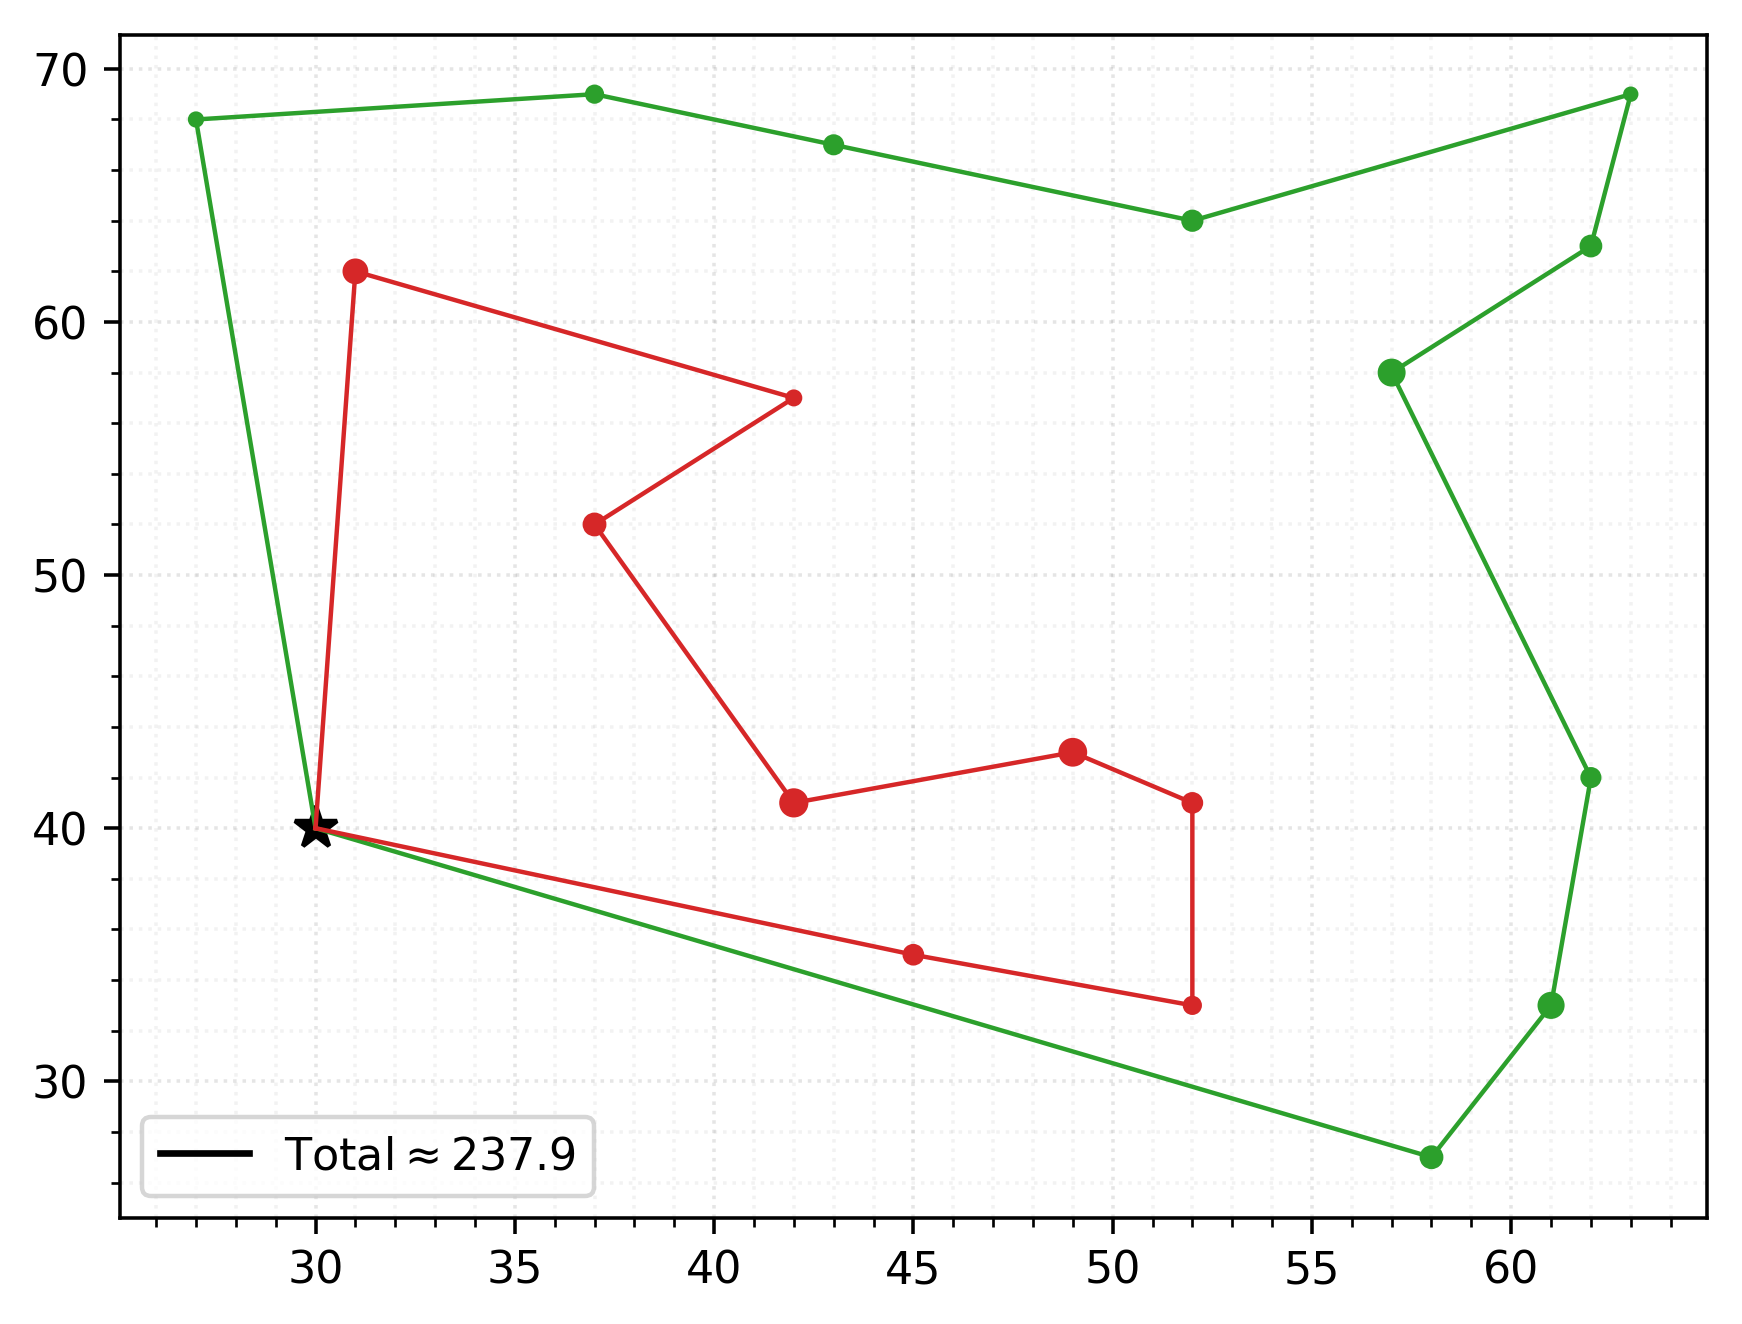
\includegraphics[width=1\textwidth]{images/savings/malosavingchico2}
		\caption{\footnotesize Ruta resultado savings para la instancia \textbf{P-n19-k2}}
		\label{fig:savings-malo-chico2}
	\end{minipage}%
	\hspace{0.03\textwidth}
	\begin{minipage}{0.35\textwidth}
		\centering
		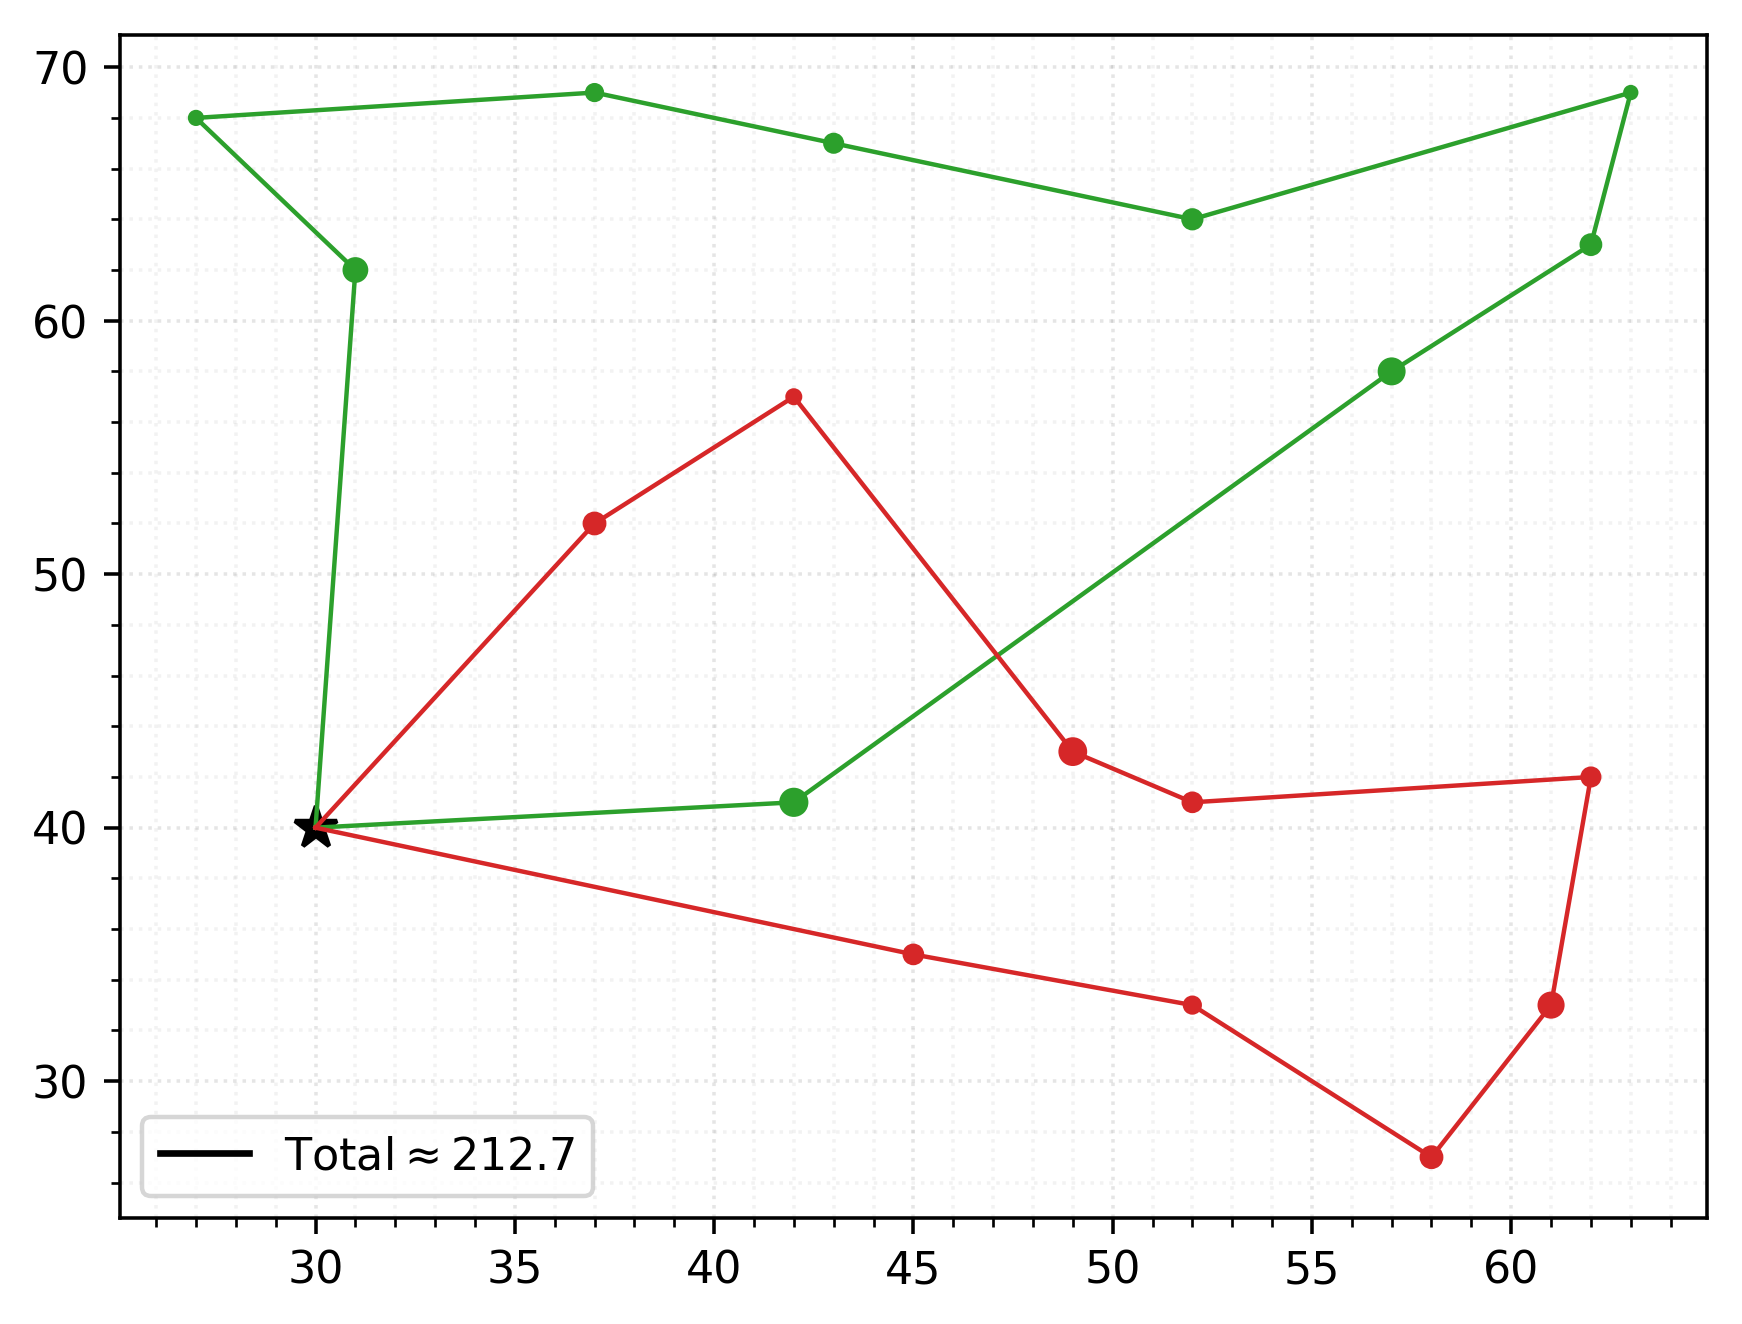
\includegraphics[width=1\textwidth]{images/savings/optimochico2}
		\caption{\footnotesize Ruta óptima para la instancia \textbf{P-n19-k2}}
		\label{fig:savings-optimo-chico2}
	\end{minipage}%
\end{figure}
\begin{figure}[H]
	\centering
	\begin{minipage}{0.35\textwidth}
		\centering
		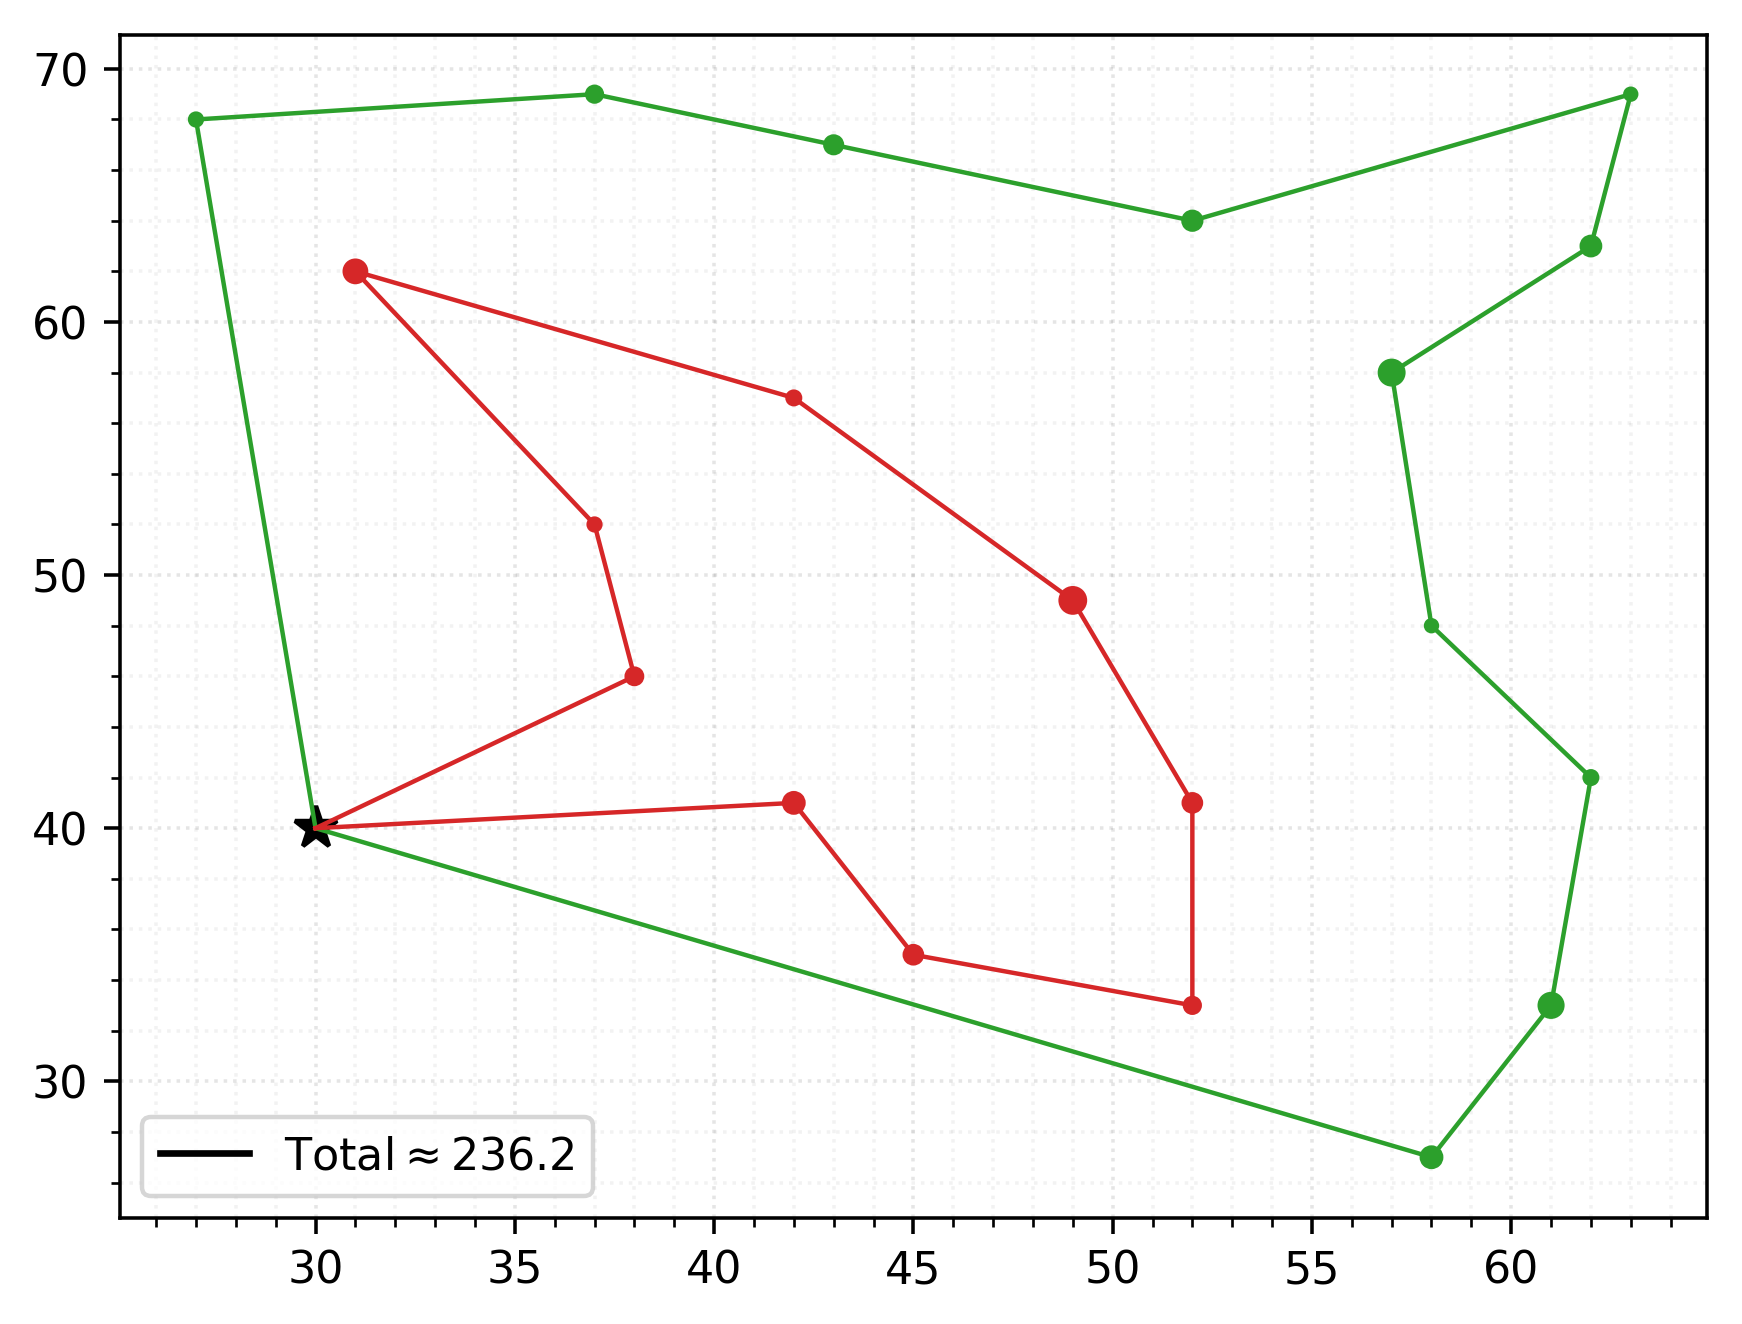
\includegraphics[width=1\textwidth]{images/savings/malosavingchico}
		\caption{\footnotesize Ruta resultado savings para la instancia \textbf{P-n21-k2}}
		\label{fig:savings-malo-chico}
	\end{minipage}%
	\hspace{0.03\textwidth}
	\begin{minipage}{0.35\textwidth}
		\centering
		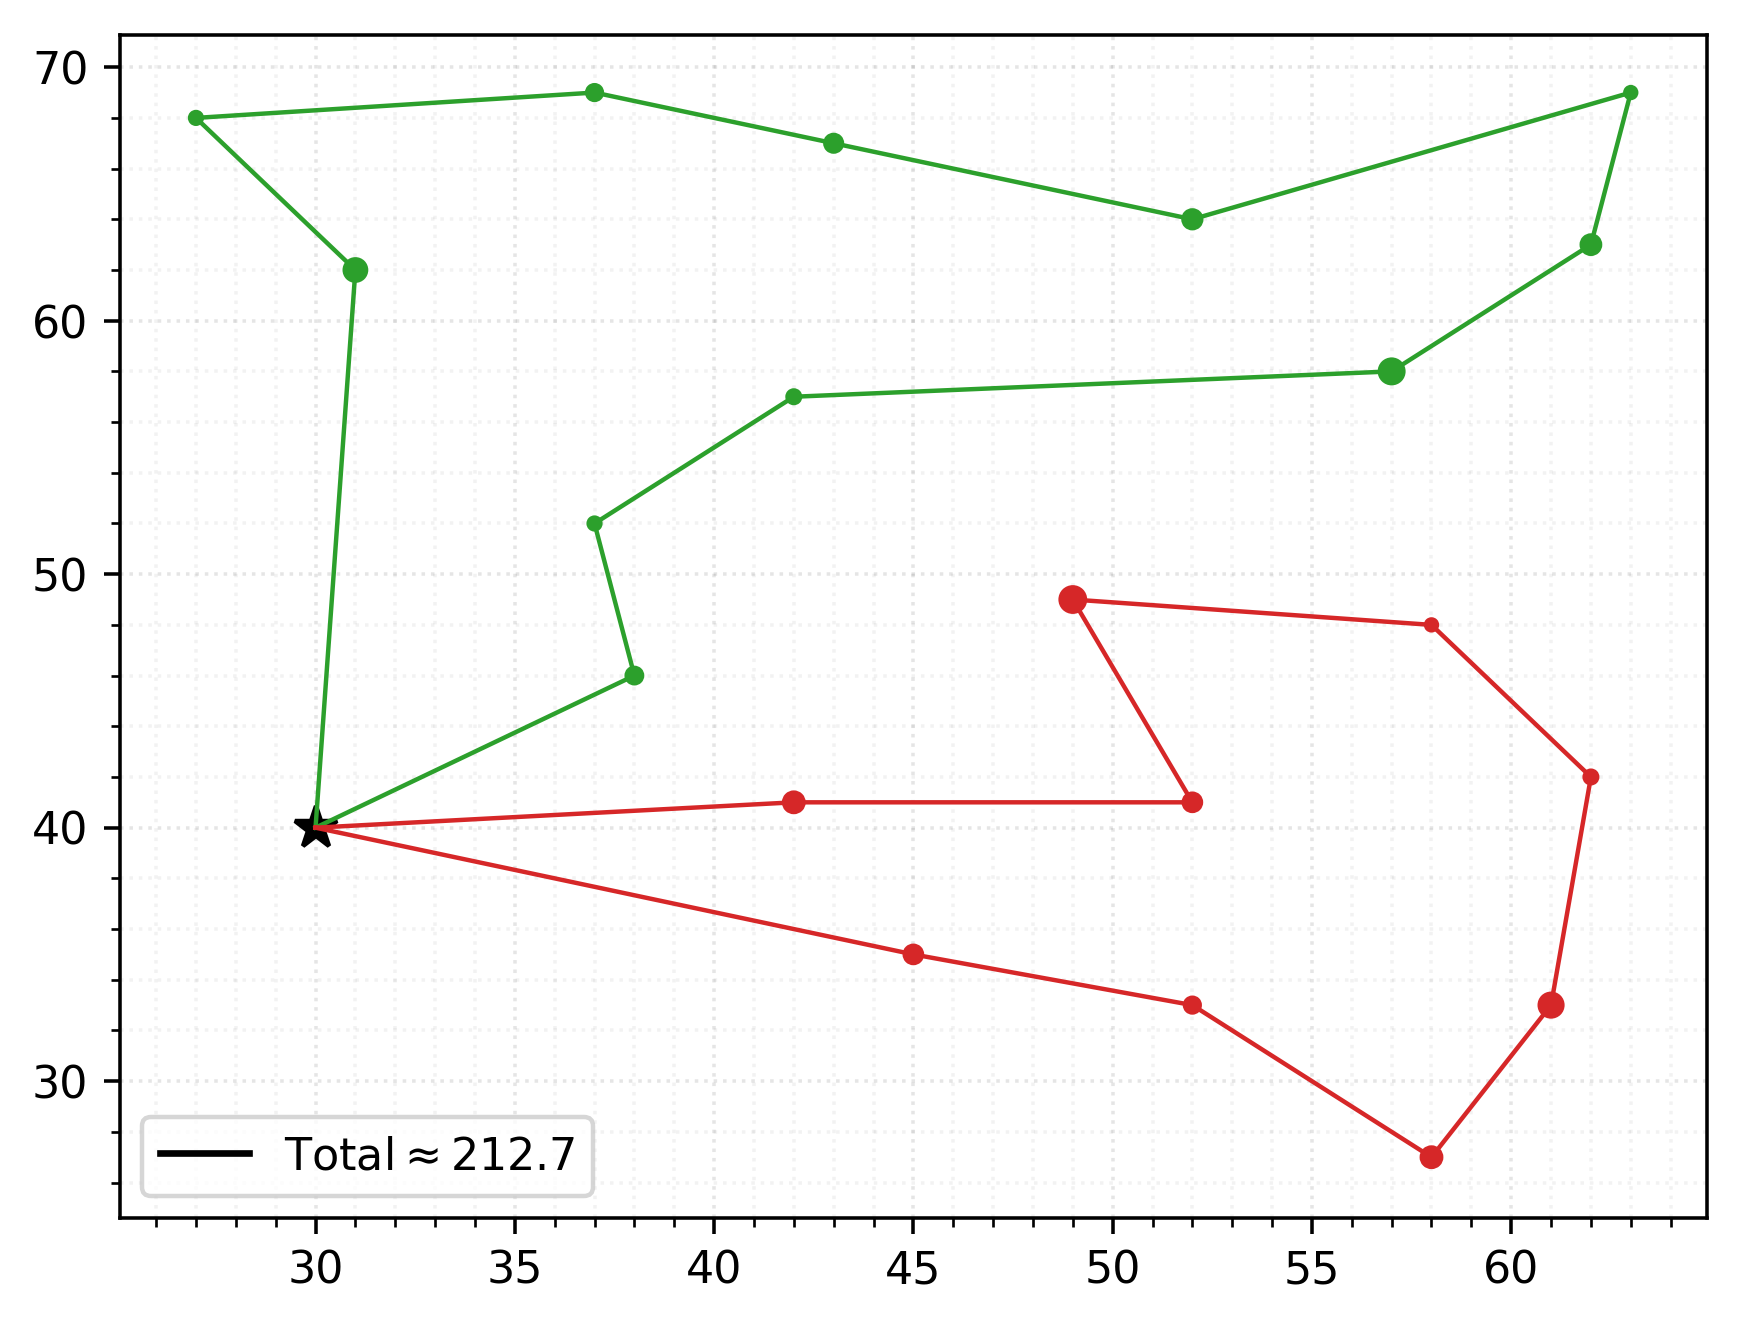
\includegraphics[width=1\textwidth]{images/savings/optimochico}
		\caption{\footnotesize Ruta óptima para la instancia \textbf{P-n21-k2}}
		\label{fig:savings-optimo-chico}
	\end{minipage}%
\end{figure}
Si bien las soluciones óptimas tienen una forma de ruta distinta entre sí, podemos notar que saving en ambos casos dio esta forma de ruta. 
\par Otro caso que pertenecerá al mismo data set que los últimos dos, con los que experimentaremos luego es el de la figura \ref{fig:savings-malo-grande}. Aquí es más marcada la diferencia entre ambos recorridos, siendo savings un 15.2\% peor que la óptima.
\begin{figure}[H]
	\centering
	\begin{minipage}{0.35\textwidth}
		\centering
		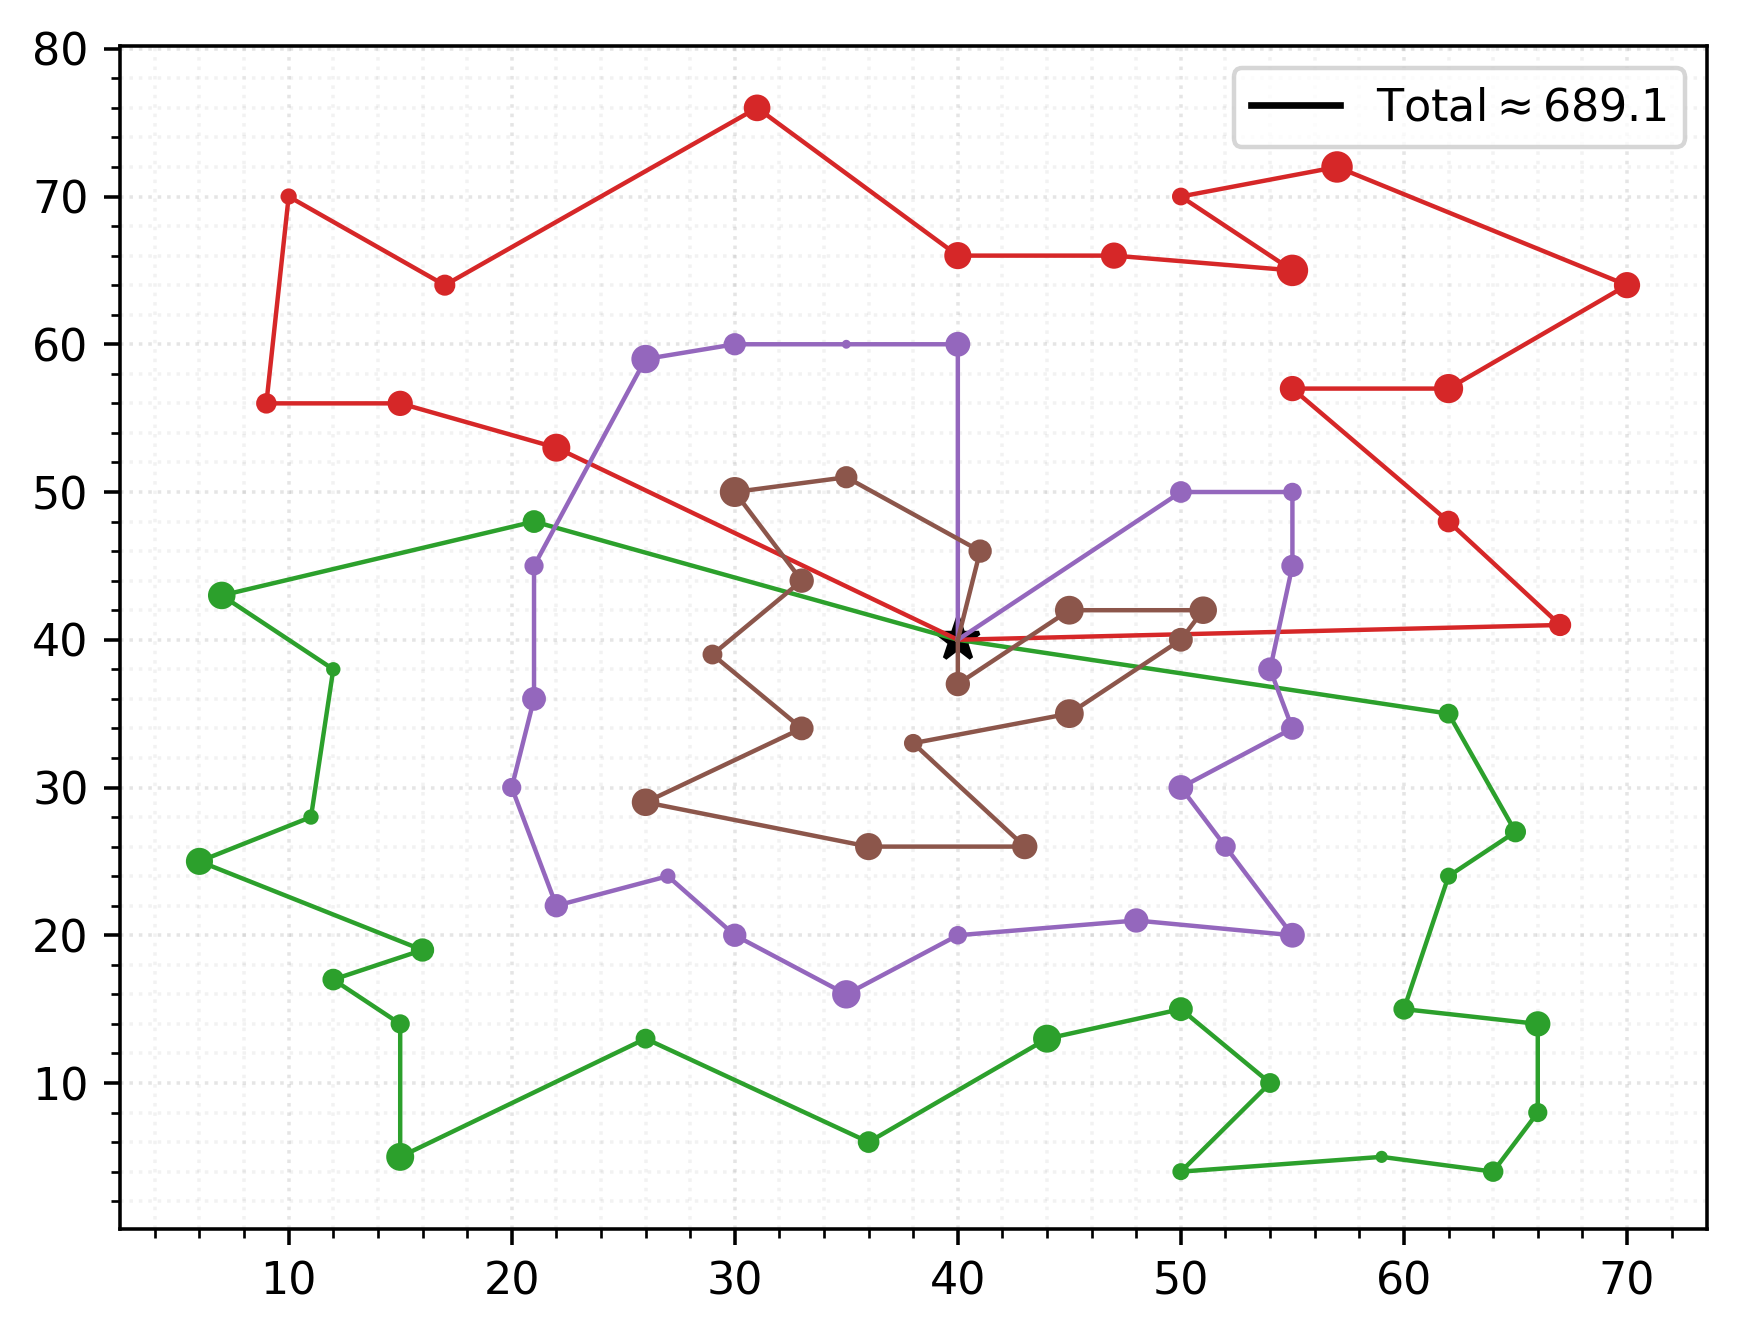
\includegraphics[width=1\textwidth]{images/savings/malosavinggrande}
		\caption{\footnotesize Ruta resultado savings para la instancia \textbf{P-n76-k4}}
		\label{fig:savings-malo-grande}
	\end{minipage}%
	\hspace{0.03\textwidth}
	\begin{minipage}{0.35\textwidth}
		\centering
		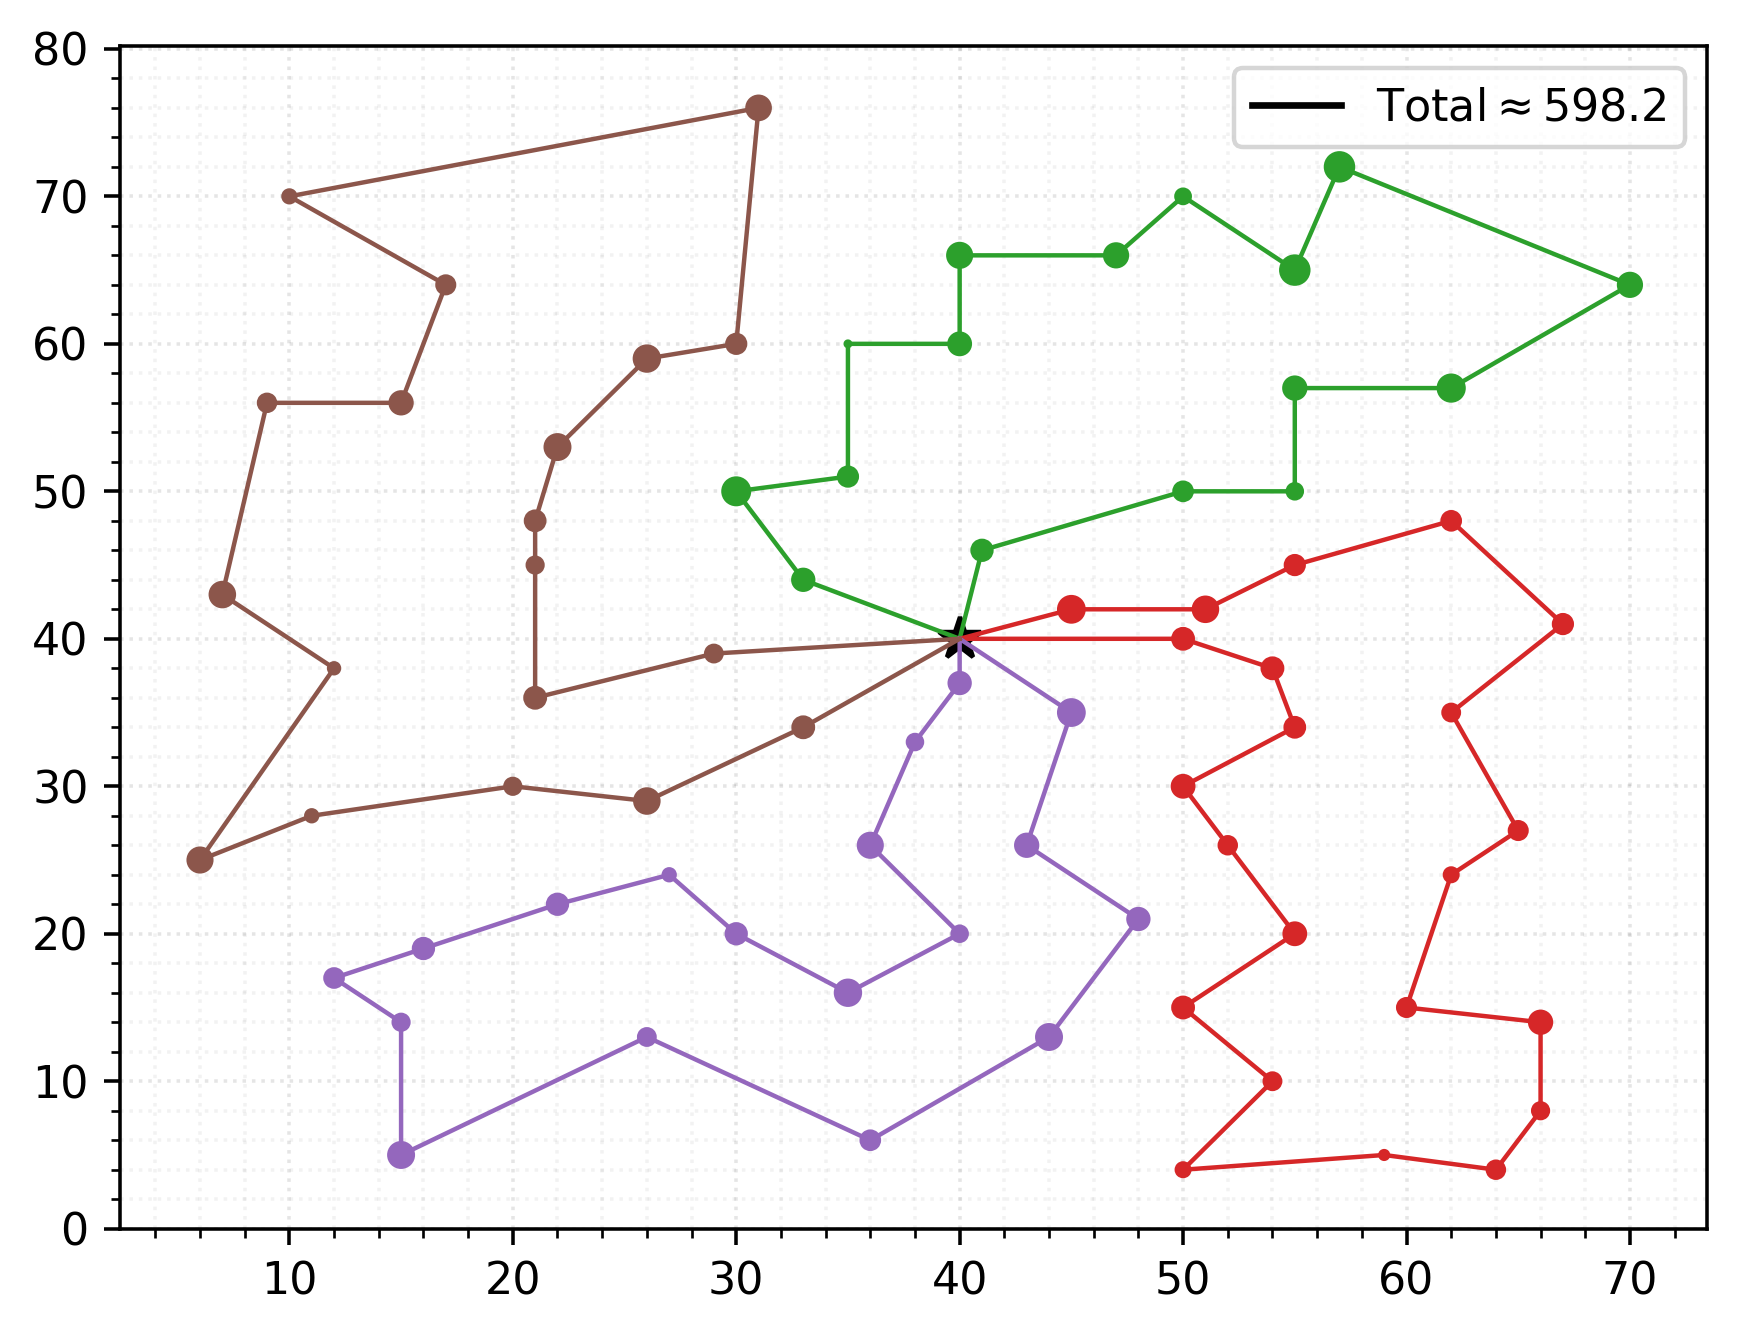
\includegraphics[width=1\textwidth]{images/savings/optimogrande}
		\caption{\footnotesize Ruta óptima para la instancia \textbf{P-n76-k4}}
		\label{fig:savings-optimo-grande}
	\end{minipage}%
\end{figure}


\section{Experimentación}

\subsection{Aclaraciones}

Para la siguiente experimentación, se optó por tomar dos casos distintos para graficar la performance de cada heurística:

\begin{itemize}
\item Medición de performance en base a tamaño del grafo.
\item Medición de performance en base a distribución del grafo.
\end{itemize}

\subsubsection{Medición en base a tamaño del grafo}
Para realizar el siguiente experimento, se tomaron datasets con distintas distribuciones del mismo tamaño y se tomó el promedio de ejecución para cada uno de ellos en base a 50 ejecuciones. En base a los resultados obtenidos, se seleccionó el mejor caso y se realizaron pruebas sobre datasets incrementando el tamaño.

\vskip 8pt

El punto de partida es un dataset de tamaño n = 45 ya que dicho tamaño se encontraba disponible para todos los tipos de datasets a experimentar.

\subsubsection{Medición en base a tamaño del grafo}
En base al mejor caso encontrado para el punto anterior, se utilizaron las demás instancias para mostrar como la distribución del grafo afecta la performance del mismo.

\section{Experimentación}

\subsection{Aclaraciones}

Para la siguiente experimentación, se optó por tomar dos casos distintos para graficar la performance de cada heurística:

\begin{itemize}
\item Medición de performance en base a tamaño del grafo.
\item Medición de performance en base a distribución del grafo.
\end{itemize}

\subsubsection{Medición en base a tamaño del grafo}
Para realizar el siguiente experimento, se tomaron datasets con distintas distribuciones del mismo tamaño y se tomó el promedio de ejecución para cada uno de ellos en base a 50 ejecuciones. En base a los resultados obtenidos, se seleccionó el mejor caso y se realizaron pruebas sobre datasets incrementando el tamaño.

\vskip 8pt

El punto de partida es un dataset de tamaño n = 45 ya que dicho tamaño se encontraba disponible para todos los tipos de datasets a experimentar.

\subsubsection{Medición en base a tamaño del grafo}
En base al mejor caso encontrado para el punto anterior, se utilizaron las demás instancias para mostrar como la distribución del grafo afecta la performance del mismo.

\section{Experimentación}

\subsection{Aclaraciones}

Para la siguiente experimentación, se optó por tomar dos casos distintos para graficar la performance de cada heurística:

\begin{itemize}
\item Medición de performance en base a tamaño del grafo.
\item Medición de performance en base a distribución del grafo.
\end{itemize}

\subsubsection{Medición en base a tamaño del grafo}
Para realizar el siguiente experimento, se tomaron datasets con distintas distribuciones del mismo tamaño y se tomó el promedio de ejecución para cada uno de ellos en base a 50 ejecuciones. En base a los resultados obtenidos, se seleccionó el mejor caso y se realizaron pruebas sobre datasets incrementando el tamaño.

\vskip 8pt

El punto de partida es un dataset de tamaño n = 45 ya que dicho tamaño se encontraba disponible para todos los tipos de datasets a experimentar.

\subsubsection{Medición en base a tamaño del grafo}
En base al mejor caso encontrado para el punto anterior, se utilizaron las demás instancias para mostrar como la distribución del grafo afecta la performance del mismo.

\input{sections/savings/experimentacion}
\input{sections/greedy/experimentacion}
\input{sections/sweep/experimentacion}
\input{sections/kmeans/experimentacion}
\input{sections/annealing/experimentacion}


\section{Experimentación}

\subsection{Aclaraciones}

Para la siguiente experimentación, se optó por tomar dos casos distintos para graficar la performance de cada heurística:

\begin{itemize}
\item Medición de performance en base a tamaño del grafo.
\item Medición de performance en base a distribución del grafo.
\end{itemize}

\subsubsection{Medición en base a tamaño del grafo}
Para realizar el siguiente experimento, se tomaron datasets con distintas distribuciones del mismo tamaño y se tomó el promedio de ejecución para cada uno de ellos en base a 50 ejecuciones. En base a los resultados obtenidos, se seleccionó el mejor caso y se realizaron pruebas sobre datasets incrementando el tamaño.

\vskip 8pt

El punto de partida es un dataset de tamaño n = 45 ya que dicho tamaño se encontraba disponible para todos los tipos de datasets a experimentar.

\subsubsection{Medición en base a tamaño del grafo}
En base al mejor caso encontrado para el punto anterior, se utilizaron las demás instancias para mostrar como la distribución del grafo afecta la performance del mismo.

\input{sections/savings/experimentacion}
\input{sections/greedy/experimentacion}
\input{sections/sweep/experimentacion}
\input{sections/kmeans/experimentacion}
\input{sections/annealing/experimentacion}


\section{Experimentación}

\subsection{Aclaraciones}

Para la siguiente experimentación, se optó por tomar dos casos distintos para graficar la performance de cada heurística:

\begin{itemize}
\item Medición de performance en base a tamaño del grafo.
\item Medición de performance en base a distribución del grafo.
\end{itemize}

\subsubsection{Medición en base a tamaño del grafo}
Para realizar el siguiente experimento, se tomaron datasets con distintas distribuciones del mismo tamaño y se tomó el promedio de ejecución para cada uno de ellos en base a 50 ejecuciones. En base a los resultados obtenidos, se seleccionó el mejor caso y se realizaron pruebas sobre datasets incrementando el tamaño.

\vskip 8pt

El punto de partida es un dataset de tamaño n = 45 ya que dicho tamaño se encontraba disponible para todos los tipos de datasets a experimentar.

\subsubsection{Medición en base a tamaño del grafo}
En base al mejor caso encontrado para el punto anterior, se utilizaron las demás instancias para mostrar como la distribución del grafo afecta la performance del mismo.

\input{sections/savings/experimentacion}
\input{sections/greedy/experimentacion}
\input{sections/sweep/experimentacion}
\input{sections/kmeans/experimentacion}
\input{sections/annealing/experimentacion}


\section{Experimentación}

\subsection{Aclaraciones}

Para la siguiente experimentación, se optó por tomar dos casos distintos para graficar la performance de cada heurística:

\begin{itemize}
\item Medición de performance en base a tamaño del grafo.
\item Medición de performance en base a distribución del grafo.
\end{itemize}

\subsubsection{Medición en base a tamaño del grafo}
Para realizar el siguiente experimento, se tomaron datasets con distintas distribuciones del mismo tamaño y se tomó el promedio de ejecución para cada uno de ellos en base a 50 ejecuciones. En base a los resultados obtenidos, se seleccionó el mejor caso y se realizaron pruebas sobre datasets incrementando el tamaño.

\vskip 8pt

El punto de partida es un dataset de tamaño n = 45 ya que dicho tamaño se encontraba disponible para todos los tipos de datasets a experimentar.

\subsubsection{Medición en base a tamaño del grafo}
En base al mejor caso encontrado para el punto anterior, se utilizaron las demás instancias para mostrar como la distribución del grafo afecta la performance del mismo.

\input{sections/savings/experimentacion}
\input{sections/greedy/experimentacion}
\input{sections/sweep/experimentacion}
\input{sections/kmeans/experimentacion}
\input{sections/annealing/experimentacion}


\section{Experimentación}

\subsection{Aclaraciones}

Para la siguiente experimentación, se optó por tomar dos casos distintos para graficar la performance de cada heurística:

\begin{itemize}
\item Medición de performance en base a tamaño del grafo.
\item Medición de performance en base a distribución del grafo.
\end{itemize}

\subsubsection{Medición en base a tamaño del grafo}
Para realizar el siguiente experimento, se tomaron datasets con distintas distribuciones del mismo tamaño y se tomó el promedio de ejecución para cada uno de ellos en base a 50 ejecuciones. En base a los resultados obtenidos, se seleccionó el mejor caso y se realizaron pruebas sobre datasets incrementando el tamaño.

\vskip 8pt

El punto de partida es un dataset de tamaño n = 45 ya que dicho tamaño se encontraba disponible para todos los tipos de datasets a experimentar.

\subsubsection{Medición en base a tamaño del grafo}
En base al mejor caso encontrado para el punto anterior, se utilizaron las demás instancias para mostrar como la distribución del grafo afecta la performance del mismo.

\input{sections/savings/experimentacion}
\input{sections/greedy/experimentacion}
\input{sections/sweep/experimentacion}
\input{sections/kmeans/experimentacion}
\input{sections/annealing/experimentacion}




\section{Experimentación}

\subsection{Aclaraciones}

Para la siguiente experimentación, se optó por tomar dos casos distintos para graficar la performance de cada heurística:

\begin{itemize}
\item Medición de performance en base a tamaño del grafo.
\item Medición de performance en base a distribución del grafo.
\end{itemize}

\subsubsection{Medición en base a tamaño del grafo}
Para realizar el siguiente experimento, se tomaron datasets con distintas distribuciones del mismo tamaño y se tomó el promedio de ejecución para cada uno de ellos en base a 50 ejecuciones. En base a los resultados obtenidos, se seleccionó el mejor caso y se realizaron pruebas sobre datasets incrementando el tamaño.

\vskip 8pt

El punto de partida es un dataset de tamaño n = 45 ya que dicho tamaño se encontraba disponible para todos los tipos de datasets a experimentar.

\subsubsection{Medición en base a tamaño del grafo}
En base al mejor caso encontrado para el punto anterior, se utilizaron las demás instancias para mostrar como la distribución del grafo afecta la performance del mismo.

\section{Experimentación}

\subsection{Aclaraciones}

Para la siguiente experimentación, se optó por tomar dos casos distintos para graficar la performance de cada heurística:

\begin{itemize}
\item Medición de performance en base a tamaño del grafo.
\item Medición de performance en base a distribución del grafo.
\end{itemize}

\subsubsection{Medición en base a tamaño del grafo}
Para realizar el siguiente experimento, se tomaron datasets con distintas distribuciones del mismo tamaño y se tomó el promedio de ejecución para cada uno de ellos en base a 50 ejecuciones. En base a los resultados obtenidos, se seleccionó el mejor caso y se realizaron pruebas sobre datasets incrementando el tamaño.

\vskip 8pt

El punto de partida es un dataset de tamaño n = 45 ya que dicho tamaño se encontraba disponible para todos los tipos de datasets a experimentar.

\subsubsection{Medición en base a tamaño del grafo}
En base al mejor caso encontrado para el punto anterior, se utilizaron las demás instancias para mostrar como la distribución del grafo afecta la performance del mismo.

\input{sections/savings/experimentacion}
\input{sections/greedy/experimentacion}
\input{sections/sweep/experimentacion}
\input{sections/kmeans/experimentacion}
\input{sections/annealing/experimentacion}


\section{Experimentación}

\subsection{Aclaraciones}

Para la siguiente experimentación, se optó por tomar dos casos distintos para graficar la performance de cada heurística:

\begin{itemize}
\item Medición de performance en base a tamaño del grafo.
\item Medición de performance en base a distribución del grafo.
\end{itemize}

\subsubsection{Medición en base a tamaño del grafo}
Para realizar el siguiente experimento, se tomaron datasets con distintas distribuciones del mismo tamaño y se tomó el promedio de ejecución para cada uno de ellos en base a 50 ejecuciones. En base a los resultados obtenidos, se seleccionó el mejor caso y se realizaron pruebas sobre datasets incrementando el tamaño.

\vskip 8pt

El punto de partida es un dataset de tamaño n = 45 ya que dicho tamaño se encontraba disponible para todos los tipos de datasets a experimentar.

\subsubsection{Medición en base a tamaño del grafo}
En base al mejor caso encontrado para el punto anterior, se utilizaron las demás instancias para mostrar como la distribución del grafo afecta la performance del mismo.

\input{sections/savings/experimentacion}
\input{sections/greedy/experimentacion}
\input{sections/sweep/experimentacion}
\input{sections/kmeans/experimentacion}
\input{sections/annealing/experimentacion}


\section{Experimentación}

\subsection{Aclaraciones}

Para la siguiente experimentación, se optó por tomar dos casos distintos para graficar la performance de cada heurística:

\begin{itemize}
\item Medición de performance en base a tamaño del grafo.
\item Medición de performance en base a distribución del grafo.
\end{itemize}

\subsubsection{Medición en base a tamaño del grafo}
Para realizar el siguiente experimento, se tomaron datasets con distintas distribuciones del mismo tamaño y se tomó el promedio de ejecución para cada uno de ellos en base a 50 ejecuciones. En base a los resultados obtenidos, se seleccionó el mejor caso y se realizaron pruebas sobre datasets incrementando el tamaño.

\vskip 8pt

El punto de partida es un dataset de tamaño n = 45 ya que dicho tamaño se encontraba disponible para todos los tipos de datasets a experimentar.

\subsubsection{Medición en base a tamaño del grafo}
En base al mejor caso encontrado para el punto anterior, se utilizaron las demás instancias para mostrar como la distribución del grafo afecta la performance del mismo.

\input{sections/savings/experimentacion}
\input{sections/greedy/experimentacion}
\input{sections/sweep/experimentacion}
\input{sections/kmeans/experimentacion}
\input{sections/annealing/experimentacion}


\section{Experimentación}

\subsection{Aclaraciones}

Para la siguiente experimentación, se optó por tomar dos casos distintos para graficar la performance de cada heurística:

\begin{itemize}
\item Medición de performance en base a tamaño del grafo.
\item Medición de performance en base a distribución del grafo.
\end{itemize}

\subsubsection{Medición en base a tamaño del grafo}
Para realizar el siguiente experimento, se tomaron datasets con distintas distribuciones del mismo tamaño y se tomó el promedio de ejecución para cada uno de ellos en base a 50 ejecuciones. En base a los resultados obtenidos, se seleccionó el mejor caso y se realizaron pruebas sobre datasets incrementando el tamaño.

\vskip 8pt

El punto de partida es un dataset de tamaño n = 45 ya que dicho tamaño se encontraba disponible para todos los tipos de datasets a experimentar.

\subsubsection{Medición en base a tamaño del grafo}
En base al mejor caso encontrado para el punto anterior, se utilizaron las demás instancias para mostrar como la distribución del grafo afecta la performance del mismo.

\input{sections/savings/experimentacion}
\input{sections/greedy/experimentacion}
\input{sections/sweep/experimentacion}
\input{sections/kmeans/experimentacion}
\input{sections/annealing/experimentacion}


\section{Experimentación}

\subsection{Aclaraciones}

Para la siguiente experimentación, se optó por tomar dos casos distintos para graficar la performance de cada heurística:

\begin{itemize}
\item Medición de performance en base a tamaño del grafo.
\item Medición de performance en base a distribución del grafo.
\end{itemize}

\subsubsection{Medición en base a tamaño del grafo}
Para realizar el siguiente experimento, se tomaron datasets con distintas distribuciones del mismo tamaño y se tomó el promedio de ejecución para cada uno de ellos en base a 50 ejecuciones. En base a los resultados obtenidos, se seleccionó el mejor caso y se realizaron pruebas sobre datasets incrementando el tamaño.

\vskip 8pt

El punto de partida es un dataset de tamaño n = 45 ya que dicho tamaño se encontraba disponible para todos los tipos de datasets a experimentar.

\subsubsection{Medición en base a tamaño del grafo}
En base al mejor caso encontrado para el punto anterior, se utilizaron las demás instancias para mostrar como la distribución del grafo afecta la performance del mismo.

\input{sections/savings/experimentacion}
\input{sections/greedy/experimentacion}
\input{sections/sweep/experimentacion}
\input{sections/kmeans/experimentacion}
\input{sections/annealing/experimentacion}




\section{Experimentación}

\subsection{Aclaraciones}

Para la siguiente experimentación, se optó por tomar dos casos distintos para graficar la performance de cada heurística:

\begin{itemize}
\item Medición de performance en base a tamaño del grafo.
\item Medición de performance en base a distribución del grafo.
\end{itemize}

\subsubsection{Medición en base a tamaño del grafo}
Para realizar el siguiente experimento, se tomaron datasets con distintas distribuciones del mismo tamaño y se tomó el promedio de ejecución para cada uno de ellos en base a 50 ejecuciones. En base a los resultados obtenidos, se seleccionó el mejor caso y se realizaron pruebas sobre datasets incrementando el tamaño.

\vskip 8pt

El punto de partida es un dataset de tamaño n = 45 ya que dicho tamaño se encontraba disponible para todos los tipos de datasets a experimentar.

\subsubsection{Medición en base a tamaño del grafo}
En base al mejor caso encontrado para el punto anterior, se utilizaron las demás instancias para mostrar como la distribución del grafo afecta la performance del mismo.

\section{Experimentación}

\subsection{Aclaraciones}

Para la siguiente experimentación, se optó por tomar dos casos distintos para graficar la performance de cada heurística:

\begin{itemize}
\item Medición de performance en base a tamaño del grafo.
\item Medición de performance en base a distribución del grafo.
\end{itemize}

\subsubsection{Medición en base a tamaño del grafo}
Para realizar el siguiente experimento, se tomaron datasets con distintas distribuciones del mismo tamaño y se tomó el promedio de ejecución para cada uno de ellos en base a 50 ejecuciones. En base a los resultados obtenidos, se seleccionó el mejor caso y se realizaron pruebas sobre datasets incrementando el tamaño.

\vskip 8pt

El punto de partida es un dataset de tamaño n = 45 ya que dicho tamaño se encontraba disponible para todos los tipos de datasets a experimentar.

\subsubsection{Medición en base a tamaño del grafo}
En base al mejor caso encontrado para el punto anterior, se utilizaron las demás instancias para mostrar como la distribución del grafo afecta la performance del mismo.

\input{sections/savings/experimentacion}
\input{sections/greedy/experimentacion}
\input{sections/sweep/experimentacion}
\input{sections/kmeans/experimentacion}
\input{sections/annealing/experimentacion}


\section{Experimentación}

\subsection{Aclaraciones}

Para la siguiente experimentación, se optó por tomar dos casos distintos para graficar la performance de cada heurística:

\begin{itemize}
\item Medición de performance en base a tamaño del grafo.
\item Medición de performance en base a distribución del grafo.
\end{itemize}

\subsubsection{Medición en base a tamaño del grafo}
Para realizar el siguiente experimento, se tomaron datasets con distintas distribuciones del mismo tamaño y se tomó el promedio de ejecución para cada uno de ellos en base a 50 ejecuciones. En base a los resultados obtenidos, se seleccionó el mejor caso y se realizaron pruebas sobre datasets incrementando el tamaño.

\vskip 8pt

El punto de partida es un dataset de tamaño n = 45 ya que dicho tamaño se encontraba disponible para todos los tipos de datasets a experimentar.

\subsubsection{Medición en base a tamaño del grafo}
En base al mejor caso encontrado para el punto anterior, se utilizaron las demás instancias para mostrar como la distribución del grafo afecta la performance del mismo.

\input{sections/savings/experimentacion}
\input{sections/greedy/experimentacion}
\input{sections/sweep/experimentacion}
\input{sections/kmeans/experimentacion}
\input{sections/annealing/experimentacion}


\section{Experimentación}

\subsection{Aclaraciones}

Para la siguiente experimentación, se optó por tomar dos casos distintos para graficar la performance de cada heurística:

\begin{itemize}
\item Medición de performance en base a tamaño del grafo.
\item Medición de performance en base a distribución del grafo.
\end{itemize}

\subsubsection{Medición en base a tamaño del grafo}
Para realizar el siguiente experimento, se tomaron datasets con distintas distribuciones del mismo tamaño y se tomó el promedio de ejecución para cada uno de ellos en base a 50 ejecuciones. En base a los resultados obtenidos, se seleccionó el mejor caso y se realizaron pruebas sobre datasets incrementando el tamaño.

\vskip 8pt

El punto de partida es un dataset de tamaño n = 45 ya que dicho tamaño se encontraba disponible para todos los tipos de datasets a experimentar.

\subsubsection{Medición en base a tamaño del grafo}
En base al mejor caso encontrado para el punto anterior, se utilizaron las demás instancias para mostrar como la distribución del grafo afecta la performance del mismo.

\input{sections/savings/experimentacion}
\input{sections/greedy/experimentacion}
\input{sections/sweep/experimentacion}
\input{sections/kmeans/experimentacion}
\input{sections/annealing/experimentacion}


\section{Experimentación}

\subsection{Aclaraciones}

Para la siguiente experimentación, se optó por tomar dos casos distintos para graficar la performance de cada heurística:

\begin{itemize}
\item Medición de performance en base a tamaño del grafo.
\item Medición de performance en base a distribución del grafo.
\end{itemize}

\subsubsection{Medición en base a tamaño del grafo}
Para realizar el siguiente experimento, se tomaron datasets con distintas distribuciones del mismo tamaño y se tomó el promedio de ejecución para cada uno de ellos en base a 50 ejecuciones. En base a los resultados obtenidos, se seleccionó el mejor caso y se realizaron pruebas sobre datasets incrementando el tamaño.

\vskip 8pt

El punto de partida es un dataset de tamaño n = 45 ya que dicho tamaño se encontraba disponible para todos los tipos de datasets a experimentar.

\subsubsection{Medición en base a tamaño del grafo}
En base al mejor caso encontrado para el punto anterior, se utilizaron las demás instancias para mostrar como la distribución del grafo afecta la performance del mismo.

\input{sections/savings/experimentacion}
\input{sections/greedy/experimentacion}
\input{sections/sweep/experimentacion}
\input{sections/kmeans/experimentacion}
\input{sections/annealing/experimentacion}


\section{Experimentación}

\subsection{Aclaraciones}

Para la siguiente experimentación, se optó por tomar dos casos distintos para graficar la performance de cada heurística:

\begin{itemize}
\item Medición de performance en base a tamaño del grafo.
\item Medición de performance en base a distribución del grafo.
\end{itemize}

\subsubsection{Medición en base a tamaño del grafo}
Para realizar el siguiente experimento, se tomaron datasets con distintas distribuciones del mismo tamaño y se tomó el promedio de ejecución para cada uno de ellos en base a 50 ejecuciones. En base a los resultados obtenidos, se seleccionó el mejor caso y se realizaron pruebas sobre datasets incrementando el tamaño.

\vskip 8pt

El punto de partida es un dataset de tamaño n = 45 ya que dicho tamaño se encontraba disponible para todos los tipos de datasets a experimentar.

\subsubsection{Medición en base a tamaño del grafo}
En base al mejor caso encontrado para el punto anterior, se utilizaron las demás instancias para mostrar como la distribución del grafo afecta la performance del mismo.

\input{sections/savings/experimentacion}
\input{sections/greedy/experimentacion}
\input{sections/sweep/experimentacion}
\input{sections/kmeans/experimentacion}
\input{sections/annealing/experimentacion}




\section{Experimentación}

\subsection{Aclaraciones}

Para la siguiente experimentación, se optó por tomar dos casos distintos para graficar la performance de cada heurística:

\begin{itemize}
\item Medición de performance en base a tamaño del grafo.
\item Medición de performance en base a distribución del grafo.
\end{itemize}

\subsubsection{Medición en base a tamaño del grafo}
Para realizar el siguiente experimento, se tomaron datasets con distintas distribuciones del mismo tamaño y se tomó el promedio de ejecución para cada uno de ellos en base a 50 ejecuciones. En base a los resultados obtenidos, se seleccionó el mejor caso y se realizaron pruebas sobre datasets incrementando el tamaño.

\vskip 8pt

El punto de partida es un dataset de tamaño n = 45 ya que dicho tamaño se encontraba disponible para todos los tipos de datasets a experimentar.

\subsubsection{Medición en base a tamaño del grafo}
En base al mejor caso encontrado para el punto anterior, se utilizaron las demás instancias para mostrar como la distribución del grafo afecta la performance del mismo.

\section{Experimentación}

\subsection{Aclaraciones}

Para la siguiente experimentación, se optó por tomar dos casos distintos para graficar la performance de cada heurística:

\begin{itemize}
\item Medición de performance en base a tamaño del grafo.
\item Medición de performance en base a distribución del grafo.
\end{itemize}

\subsubsection{Medición en base a tamaño del grafo}
Para realizar el siguiente experimento, se tomaron datasets con distintas distribuciones del mismo tamaño y se tomó el promedio de ejecución para cada uno de ellos en base a 50 ejecuciones. En base a los resultados obtenidos, se seleccionó el mejor caso y se realizaron pruebas sobre datasets incrementando el tamaño.

\vskip 8pt

El punto de partida es un dataset de tamaño n = 45 ya que dicho tamaño se encontraba disponible para todos los tipos de datasets a experimentar.

\subsubsection{Medición en base a tamaño del grafo}
En base al mejor caso encontrado para el punto anterior, se utilizaron las demás instancias para mostrar como la distribución del grafo afecta la performance del mismo.

\input{sections/savings/experimentacion}
\input{sections/greedy/experimentacion}
\input{sections/sweep/experimentacion}
\input{sections/kmeans/experimentacion}
\input{sections/annealing/experimentacion}


\section{Experimentación}

\subsection{Aclaraciones}

Para la siguiente experimentación, se optó por tomar dos casos distintos para graficar la performance de cada heurística:

\begin{itemize}
\item Medición de performance en base a tamaño del grafo.
\item Medición de performance en base a distribución del grafo.
\end{itemize}

\subsubsection{Medición en base a tamaño del grafo}
Para realizar el siguiente experimento, se tomaron datasets con distintas distribuciones del mismo tamaño y se tomó el promedio de ejecución para cada uno de ellos en base a 50 ejecuciones. En base a los resultados obtenidos, se seleccionó el mejor caso y se realizaron pruebas sobre datasets incrementando el tamaño.

\vskip 8pt

El punto de partida es un dataset de tamaño n = 45 ya que dicho tamaño se encontraba disponible para todos los tipos de datasets a experimentar.

\subsubsection{Medición en base a tamaño del grafo}
En base al mejor caso encontrado para el punto anterior, se utilizaron las demás instancias para mostrar como la distribución del grafo afecta la performance del mismo.

\input{sections/savings/experimentacion}
\input{sections/greedy/experimentacion}
\input{sections/sweep/experimentacion}
\input{sections/kmeans/experimentacion}
\input{sections/annealing/experimentacion}


\section{Experimentación}

\subsection{Aclaraciones}

Para la siguiente experimentación, se optó por tomar dos casos distintos para graficar la performance de cada heurística:

\begin{itemize}
\item Medición de performance en base a tamaño del grafo.
\item Medición de performance en base a distribución del grafo.
\end{itemize}

\subsubsection{Medición en base a tamaño del grafo}
Para realizar el siguiente experimento, se tomaron datasets con distintas distribuciones del mismo tamaño y se tomó el promedio de ejecución para cada uno de ellos en base a 50 ejecuciones. En base a los resultados obtenidos, se seleccionó el mejor caso y se realizaron pruebas sobre datasets incrementando el tamaño.

\vskip 8pt

El punto de partida es un dataset de tamaño n = 45 ya que dicho tamaño se encontraba disponible para todos los tipos de datasets a experimentar.

\subsubsection{Medición en base a tamaño del grafo}
En base al mejor caso encontrado para el punto anterior, se utilizaron las demás instancias para mostrar como la distribución del grafo afecta la performance del mismo.

\input{sections/savings/experimentacion}
\input{sections/greedy/experimentacion}
\input{sections/sweep/experimentacion}
\input{sections/kmeans/experimentacion}
\input{sections/annealing/experimentacion}


\section{Experimentación}

\subsection{Aclaraciones}

Para la siguiente experimentación, se optó por tomar dos casos distintos para graficar la performance de cada heurística:

\begin{itemize}
\item Medición de performance en base a tamaño del grafo.
\item Medición de performance en base a distribución del grafo.
\end{itemize}

\subsubsection{Medición en base a tamaño del grafo}
Para realizar el siguiente experimento, se tomaron datasets con distintas distribuciones del mismo tamaño y se tomó el promedio de ejecución para cada uno de ellos en base a 50 ejecuciones. En base a los resultados obtenidos, se seleccionó el mejor caso y se realizaron pruebas sobre datasets incrementando el tamaño.

\vskip 8pt

El punto de partida es un dataset de tamaño n = 45 ya que dicho tamaño se encontraba disponible para todos los tipos de datasets a experimentar.

\subsubsection{Medición en base a tamaño del grafo}
En base al mejor caso encontrado para el punto anterior, se utilizaron las demás instancias para mostrar como la distribución del grafo afecta la performance del mismo.

\input{sections/savings/experimentacion}
\input{sections/greedy/experimentacion}
\input{sections/sweep/experimentacion}
\input{sections/kmeans/experimentacion}
\input{sections/annealing/experimentacion}


\section{Experimentación}

\subsection{Aclaraciones}

Para la siguiente experimentación, se optó por tomar dos casos distintos para graficar la performance de cada heurística:

\begin{itemize}
\item Medición de performance en base a tamaño del grafo.
\item Medición de performance en base a distribución del grafo.
\end{itemize}

\subsubsection{Medición en base a tamaño del grafo}
Para realizar el siguiente experimento, se tomaron datasets con distintas distribuciones del mismo tamaño y se tomó el promedio de ejecución para cada uno de ellos en base a 50 ejecuciones. En base a los resultados obtenidos, se seleccionó el mejor caso y se realizaron pruebas sobre datasets incrementando el tamaño.

\vskip 8pt

El punto de partida es un dataset de tamaño n = 45 ya que dicho tamaño se encontraba disponible para todos los tipos de datasets a experimentar.

\subsubsection{Medición en base a tamaño del grafo}
En base al mejor caso encontrado para el punto anterior, se utilizaron las demás instancias para mostrar como la distribución del grafo afecta la performance del mismo.

\input{sections/savings/experimentacion}
\input{sections/greedy/experimentacion}
\input{sections/sweep/experimentacion}
\input{sections/kmeans/experimentacion}
\input{sections/annealing/experimentacion}




\section{Experimentación}

\subsection{Aclaraciones}

Para la siguiente experimentación, se optó por tomar dos casos distintos para graficar la performance de cada heurística:

\begin{itemize}
\item Medición de performance en base a tamaño del grafo.
\item Medición de performance en base a distribución del grafo.
\end{itemize}

\subsubsection{Medición en base a tamaño del grafo}
Para realizar el siguiente experimento, se tomaron datasets con distintas distribuciones del mismo tamaño y se tomó el promedio de ejecución para cada uno de ellos en base a 50 ejecuciones. En base a los resultados obtenidos, se seleccionó el mejor caso y se realizaron pruebas sobre datasets incrementando el tamaño.

\vskip 8pt

El punto de partida es un dataset de tamaño n = 45 ya que dicho tamaño se encontraba disponible para todos los tipos de datasets a experimentar.

\subsubsection{Medición en base a tamaño del grafo}
En base al mejor caso encontrado para el punto anterior, se utilizaron las demás instancias para mostrar como la distribución del grafo afecta la performance del mismo.

\section{Experimentación}

\subsection{Aclaraciones}

Para la siguiente experimentación, se optó por tomar dos casos distintos para graficar la performance de cada heurística:

\begin{itemize}
\item Medición de performance en base a tamaño del grafo.
\item Medición de performance en base a distribución del grafo.
\end{itemize}

\subsubsection{Medición en base a tamaño del grafo}
Para realizar el siguiente experimento, se tomaron datasets con distintas distribuciones del mismo tamaño y se tomó el promedio de ejecución para cada uno de ellos en base a 50 ejecuciones. En base a los resultados obtenidos, se seleccionó el mejor caso y se realizaron pruebas sobre datasets incrementando el tamaño.

\vskip 8pt

El punto de partida es un dataset de tamaño n = 45 ya que dicho tamaño se encontraba disponible para todos los tipos de datasets a experimentar.

\subsubsection{Medición en base a tamaño del grafo}
En base al mejor caso encontrado para el punto anterior, se utilizaron las demás instancias para mostrar como la distribución del grafo afecta la performance del mismo.

\input{sections/savings/experimentacion}
\input{sections/greedy/experimentacion}
\input{sections/sweep/experimentacion}
\input{sections/kmeans/experimentacion}
\input{sections/annealing/experimentacion}


\section{Experimentación}

\subsection{Aclaraciones}

Para la siguiente experimentación, se optó por tomar dos casos distintos para graficar la performance de cada heurística:

\begin{itemize}
\item Medición de performance en base a tamaño del grafo.
\item Medición de performance en base a distribución del grafo.
\end{itemize}

\subsubsection{Medición en base a tamaño del grafo}
Para realizar el siguiente experimento, se tomaron datasets con distintas distribuciones del mismo tamaño y se tomó el promedio de ejecución para cada uno de ellos en base a 50 ejecuciones. En base a los resultados obtenidos, se seleccionó el mejor caso y se realizaron pruebas sobre datasets incrementando el tamaño.

\vskip 8pt

El punto de partida es un dataset de tamaño n = 45 ya que dicho tamaño se encontraba disponible para todos los tipos de datasets a experimentar.

\subsubsection{Medición en base a tamaño del grafo}
En base al mejor caso encontrado para el punto anterior, se utilizaron las demás instancias para mostrar como la distribución del grafo afecta la performance del mismo.

\input{sections/savings/experimentacion}
\input{sections/greedy/experimentacion}
\input{sections/sweep/experimentacion}
\input{sections/kmeans/experimentacion}
\input{sections/annealing/experimentacion}


\section{Experimentación}

\subsection{Aclaraciones}

Para la siguiente experimentación, se optó por tomar dos casos distintos para graficar la performance de cada heurística:

\begin{itemize}
\item Medición de performance en base a tamaño del grafo.
\item Medición de performance en base a distribución del grafo.
\end{itemize}

\subsubsection{Medición en base a tamaño del grafo}
Para realizar el siguiente experimento, se tomaron datasets con distintas distribuciones del mismo tamaño y se tomó el promedio de ejecución para cada uno de ellos en base a 50 ejecuciones. En base a los resultados obtenidos, se seleccionó el mejor caso y se realizaron pruebas sobre datasets incrementando el tamaño.

\vskip 8pt

El punto de partida es un dataset de tamaño n = 45 ya que dicho tamaño se encontraba disponible para todos los tipos de datasets a experimentar.

\subsubsection{Medición en base a tamaño del grafo}
En base al mejor caso encontrado para el punto anterior, se utilizaron las demás instancias para mostrar como la distribución del grafo afecta la performance del mismo.

\input{sections/savings/experimentacion}
\input{sections/greedy/experimentacion}
\input{sections/sweep/experimentacion}
\input{sections/kmeans/experimentacion}
\input{sections/annealing/experimentacion}


\section{Experimentación}

\subsection{Aclaraciones}

Para la siguiente experimentación, se optó por tomar dos casos distintos para graficar la performance de cada heurística:

\begin{itemize}
\item Medición de performance en base a tamaño del grafo.
\item Medición de performance en base a distribución del grafo.
\end{itemize}

\subsubsection{Medición en base a tamaño del grafo}
Para realizar el siguiente experimento, se tomaron datasets con distintas distribuciones del mismo tamaño y se tomó el promedio de ejecución para cada uno de ellos en base a 50 ejecuciones. En base a los resultados obtenidos, se seleccionó el mejor caso y se realizaron pruebas sobre datasets incrementando el tamaño.

\vskip 8pt

El punto de partida es un dataset de tamaño n = 45 ya que dicho tamaño se encontraba disponible para todos los tipos de datasets a experimentar.

\subsubsection{Medición en base a tamaño del grafo}
En base al mejor caso encontrado para el punto anterior, se utilizaron las demás instancias para mostrar como la distribución del grafo afecta la performance del mismo.

\input{sections/savings/experimentacion}
\input{sections/greedy/experimentacion}
\input{sections/sweep/experimentacion}
\input{sections/kmeans/experimentacion}
\input{sections/annealing/experimentacion}


\section{Experimentación}

\subsection{Aclaraciones}

Para la siguiente experimentación, se optó por tomar dos casos distintos para graficar la performance de cada heurística:

\begin{itemize}
\item Medición de performance en base a tamaño del grafo.
\item Medición de performance en base a distribución del grafo.
\end{itemize}

\subsubsection{Medición en base a tamaño del grafo}
Para realizar el siguiente experimento, se tomaron datasets con distintas distribuciones del mismo tamaño y se tomó el promedio de ejecución para cada uno de ellos en base a 50 ejecuciones. En base a los resultados obtenidos, se seleccionó el mejor caso y se realizaron pruebas sobre datasets incrementando el tamaño.

\vskip 8pt

El punto de partida es un dataset de tamaño n = 45 ya que dicho tamaño se encontraba disponible para todos los tipos de datasets a experimentar.

\subsubsection{Medición en base a tamaño del grafo}
En base al mejor caso encontrado para el punto anterior, se utilizaron las demás instancias para mostrar como la distribución del grafo afecta la performance del mismo.

\input{sections/savings/experimentacion}
\input{sections/greedy/experimentacion}
\input{sections/sweep/experimentacion}
\input{sections/kmeans/experimentacion}
\input{sections/annealing/experimentacion}





